\chapter{Technische Grundlagen}
\label{sec:TechnischeGrundlagen}
In diesem Kapitel werden alle nötigen technischen Grundlagen zusammengetragen. Da es sich um ein OAuth2 System handelt, wird diese Spezifikation erläutert. Zudem wird auf die Tokens eingegangen, die die Ressource Server jeweils validieren müssen. Diese sind \ac{JSON} Web Token. Dann werden die Metriken zum Messen der Performance erläutert, das Programm zum Messen dieser Werte genannt sowie das Framework zur Implementierung der Ressource Server erklärt. 

%
% Section: Der erste Abschnitt
%
\section{Grundlegende Begriffe der IT-Sicherheit}
\label{sec:GrundlegenderBegriffederIT-Sicherheit}
Im Bereich der IT-Sicherheit gibt es eine Reihe relevanter Begriffe, die regelmäßig verwendet werden.

\begin{description}
  \item[Authentifizierung:] Bei einer Authentifizierung beweist ein Nutzer seine Identität, indem er dem gegenüberliegenden System Informationen übermittelt, über die nur der Nutzer verfügen kann wie beispielsweise ein Nutzername und Passwort oder ein Token \citep{Cankaya2011}.
  \item[Autorisierung:] Eine Autorisierung findet grundsätzlich nach der Authentifizierung statt. Hier überprüft das System nach der Authentifizierung des Nutzers, ob der Nutzer über die notwendigen Rechte verfügt eine Aktion auszuführen \citep{Authorization2011}. 
  \item[Integrität:] Bei der Integrität wird verifiziert, dass Daten seit ihrer Erstellung nicht verändert wurden. Dies kann beispielsweise durch eine Signatur, die nur der Ersteller der Daten erstellen kann, gewährleistet werden \citep{connect2id:2021}.
  \item[Authentizität:] Das Ziel der Authentizität ist die Verifizierung des Erstellers der Daten \citep{connect2id:2021}. Das bedeutet, es soll möglich sein zu überprüfen, dass die Daten, die zugesendet werden, auch tatsächlich von der Person oder dem System kommen, von der man annimmt, dass sie der Urheber ist.
  \item[Validierung:] Man kann von einer Validierung sprechen, wenn die Authentizität und Integrität überprüft werden.
  \item[Zugriffskontrolle:] Zugriffskontrolle ist eine Sicherheitsfunktion, die gemeinsame Ressourcen gegen unautorisierten Zugriff schützt. Der Unterschied zwischen autorisierten und unautorisierten Zugriff wird anhand einer Zugriffskontrollrichtlinie gemacht \citep{Brose2011}. 
\end{description}

%
% Section: Der Zweite Abschnitt
%
\section{OAuth2}
\label{sec:OAuth2}
OAuth2 ist eine Spezifikation, die ursprünglich entwickelt wurde, um Dritten Zugriff auf die Daten eines sogenannten Ressource Owners zu ermöglichen, ohne dass dieser Ressource Owner dem Dritten, in der Spezifikation Client genannt, sein Nutzername und Passwort übermitteln muss \citep{oauth2:2012}. Dies wird dadurch ermöglicht, dass dem Client von einem Autorisationsserver ein Token übermittelt wird und mit diesem Token kann der Client Daten des Ressource Owners abfragen oder Aktionen im Namen des Ressource Owners durchführen. Diese Daten des Ressource Owners werden auf dem sogenannten Ressource Server gehostet.
Im Laufe der Zeit wurde diese Spezifikation erweitert, um weitere Anwendungsfälle abzudecken, wie die Spezifikation OpenID Connect, welche Single-Sign-On ermöglicht. 

\subsection{Rollen in OAuth2}
\label{subsec:OAuth2:RolleninOAuth2}
Es gibt vier verschiedene Rollen, die in OAuth2 spezifiziert sind \citep{oauth2:2012}.

\begin{description}
  \item[Ressource Owner:] Der Ressource Owner ist dazu in der Lage, Dritten Zugriff auf seine Daten zu geben oder Aktionen in seinem Namen durchzuführen. Falls der Ressource Owner eine Person ist, nennt man ihn den End-Nutzer.
  \item[Ressource Server:] Der Ressource Server hostet die geschützten Ressourcen des Ressource Owners und ist in der Lage Anfragen zu diesen Ressourcen zu beantworten, falls ein valider Token, ein sogenannter Access Token, in der Anfrage zur Ressource vorliegt.
  \item[Client:] Der Client ist diejenige Komponente, die die Ressource des Ressource Owner's von dem Ressource Servers erlangen möchte und dafür einen Access Token benötigt. 
  \item[Authorization Server:] Der Authorization Server, zu deutsch Autorisationsserver, verteilt Access Token falls sich der Ressource Owner erfolgreich authentifiziert und gegebenenfalls den Client autorisiert hat, Aktionen durchzuführen. 
\end{description}

\subsection{Erhalt von Token}
\label{subsec:OAuth2:ErhaltvonToken}

Gemäß der Spezifikation gibt es fünf verschiedene Wege, wie ein Client von einem Authorization Server einen Token erhalten kann \citep{oauth2:2012}. Im Folgenden wird nur der sogenannte Authorization Code Grant beschrieben, da die anderen vier für diese Arbeit keine Relevanz haben.\smallskip

Bei dem Authorization Code Grant wird der Ressource Owner, der einen Webbrowser verwendet, von dem Client auf den Authorization Server weitergeleitet, um den Ressource Owner zu bitten, sich bei dem Authorization Server zu authentifizieren, um dann dem Client zu autorisieren auf eine geschützte Ressource des Ressource Servers zuzugreifen \citep{oauth2:2012}. 

\begin{figure}[htbp]
  \centering
  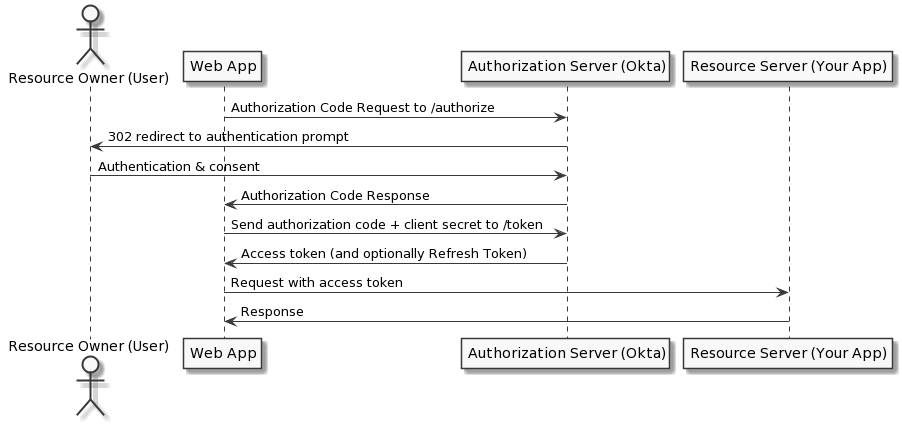
\includegraphics[width=1.0\textwidth]{gfx/oauth_auth_code_flow.png}
  \caption{Authorization Code Grant \citep{okta:2020}}
  \label{fig:chapter02:oauth_auth_code_flow}
\end{figure}

In \autoref{fig:chapter02:oauth_auth_code_flow} ist der Authorization Code Grant Flow als Sequenzdiagramm abgebildet. Es ist zu sehen, dass es Beziehungen zwischen allen vier Rollen gibt, nämlich dem Ressource Owner, dem Client, in diesem Fall als „Web App“ gekennzeichnet, dem Authorization Server, Okta, und dem Ressource Server. 
Grob kann man es sich in der Praxis so vorstellen, dass ein Nutzer eine Webapplikation (=Client) bedient und diese Webapplikation möchte, dass der Nutzer sie autorisiert, in ihrem Namen seine Adressdaten von dem Google-Konto abzufragen. In diesem Fall wäre Google der Authorization und Ressource Server. Die Webapplikation, die der Client ist, leitet also den Nutzer auf den Google-Server weiter, wo er dann aufgefordert wird sich zu authentifizieren und der Webapplikation Erlaubnis zu erteilen, Daten abzufragen. Daraufhin wird der Webbrowser des End-Nutzers zu dem Client zurückgeleitet und der Client erhält einen Token von dem Authorization Server, womit er die Ressource des End-Nutzers von dem Ressource Server abfragen kann. 

\section{JSON Web Token}
\label{sec:JSONWebToken}
Wenn ein Client einen Access Token von einem Authorization Server erhält, um Zugriff auf \ac{HTTP}-Schnittstellen des Ressource Servers zu erhalten, sind diese Token bei den heutigen Implementierungen von Autorisationsservern sogenannte \ac{JSON} Web Token, so auch bei dem Autorisationsserver von Microsoft \citep{azuread:2021}, Azure Active Directory, sowie Keycloak \citep{keycloak:2021}. \ac{JSON} ist ein leichtgewichtiges Datenaustauschformat \citep{json:2006}.\smallskip

JSON Web Token ist eine Spezifikation für Token, die beschreibt wie die Tokens aufgebaut sind und welche Inhalte sie haben \citep{jwt:2015}.
Signierte JSON Web Token sind in drei Teile unterteilt: Header, Payload und die Signatur. Die Gesamtstruktur ist in JSON dargestellt, das heißt es gibt jeweils Schlüssel-Wert-Paare in JSON. Zur Übertragung werden die JSON Web Token base64-kodiert und hierbei werden jeweils die drei Teile, also Header, Payload und Signatur, durch einen Punkt (‚.‘) voneinander getrennt \citep{jwt:2015}. 
In dem Header und Payload stehen sogenannte Claims. Ein Claim ist ein Schlüssel-Wert-Paar. Diese liefern Informationen über den Token wie zum Beispiel „exp“, kurz für „Expiration Time“, der angibt, bis wann der Token gültig ist. Einen Token, der schon abgelaufen ist, sollte der Ressource Server nicht akzeptieren. Die Namen der Schlüssel der Claims sind standardisiert. 

\begin{lstlisting}[language=C++,frame=tb,caption={Beispiel JSON Web Token},label=lst:BeispielJSONWebToken]
  {
    alg: "RS256",
    typ: "JWT",
    kid: "KaD7XcL-5_0lEdjztl8fCqrR2R-uCf1BtCyngSfI7mg"
  }.
  {
    exp: 1625764809,
    iat: 1625763009,
    jti: "7df07f70-5c50-41fd-b757-2e3faa8c50e4",
    iss: "HTTP://localhost:9080/auth/realms/sample",
    aud: "account",
    sub: "de16edd9-a654-4769-b71c-3faf34583890",
    typ: "Bearer",
    azp: "test-app",
    session_state: "a19e1f5f-4080-488f-b193-a943925d62fc",
    acr: "1",
  }.
  [signature]   
\end{lstlisting}

Obenstehend ist ein rudimentärer dekodierter JSON Web Token dargestellt. In dem \autoref{subsec:OpenIDConnect:IDToken}
wird erläutert, welche Bedeutung die einzelnen Claims haben.

\subsection{JSON Web Token Signatur}
\label{sec:JSONWebToken:JSONWebTokenSignatur}

JSON Web Tokens sind in der Regel mit dem asymmetrischen Verfahren \ac{RSA} signiert \citep{jwt:2015}. Das bedeutet, dass mittels eines privaten Schlüssels, über den
nur der Ersteller des Tokens verfügt, also der Autorisationsserver, die Signatur erzeugt wird.
Daneben gibt es einen öffentlichen Schlüssel, mit dem die Signatur überprüft werden kann.
Das heißt es ist nicht möglich, dass der Client den Token verändern kann, da dann die
Signatur nicht mehr übereinstimmt. Dadurch sind die Authentizität und die Integrität des
Tokens sichergestellt.

\subsection{JSON Web Token Key}
\label{sec:JSONWebToken:JSONWebTokenKey}
Im Falle eines durch RSA signierten JSON Web Token, ist der JSON Web Key der im JSONFormat dargestellte öffentliche Schlüssel \citep{jwk:2015}. 

\subsection{Base64 Kodierung}
\label{sec:JSONWebToken:Base64Kodierung}
JSON Web Token werden, wenn sie übertragen werden, in Base64 kodiert \citep{jwt:2015}. Base64 ist
keine Verschlüsselung und auch keine Datenkomprimierung, sondern dient vor allem dem
Zweck, dass Daten in ausschließlich ANSI-Zeichen kodiert übertragen werden, also das
irreguläre Zeichen wie Umlaute nicht mehr vorkommen, um Probleme vorzubeugen \citep{base64:2006}. 

\section{OpenID Connect}
\label{sec:OpenIDConnect}
OpenID Connect ist eine Authentifizierungsschicht, die auf der OAuth2 Spezifikation
aufbaut.
Ursprünglich wurde OAuth2 nur dazu angewandt, dass Clients im Namen des Ressource
Owners auf Daten auf dem Ressource Server durch den Erhalt eines Tokens von einem
Authorization Server zugreifen darf.
OpenID Connect baut darauf eine Authentifizierung auf, indem es in dem JSON Web Token
Claims steckt, dass den Client, der den Token erhalten hat, nachdem sich ein End-Nutzer bei
dem Authorization Server authentifiziert hat, die Möglichkeit gibt die Identität dieses End-Nutzers zu verifizieren.
Diese Art von JSON Web Token, die der Client erhält nennt sich ID Token \citep{openidconnect:2014}. 

\subsection{ID Token}
\label{subsec:OpenIDConnect:IDToken}
ID Token sind JSON Web Token, die gewisse Claims in ihrem Payload gesetzt haben \citep{openidconnect:2014}. Diese sind in \autoref{tab:idtoken} gelistet.

\begin{table}[h]
  \myfloatalign
  \begin{tabularx}{\textwidth}{|l|X|} \toprule
      \tableheadline{Claim} & \tableheadline{Beschreibung} \\ \midrule
      iss & Die Issuer-URL. Dies ist die \ac{URL} des Authorization Server, der den Token 
      erstellt hat („Herausgeber“). \\
      \midrule
      sub & Das Subject. Dies ist ein eindeutiger Identifier des Nutzers, der sich 
      authentifiziert hat. \\
      \midrule
      aud & Die Audience. Das ist der Empfänger des Tokens, also in der Regel die 
      Client-ID. \\
      \midrule
      exp & Expiration Time. Das ist der Zeitpunkt, zu dem der Token abgelaufen ist. \\
      \midrule
      iat & Issued at. Das ist der Zeitpunkt, zu dem der Token herausgegeben wurde. \\
      \bottomrule
  \end{tabularx}
  \caption[ID Token]{ID Token.}
  \label{tab:idtoken}

  \bigskip
In \autoref{tab:idtoken} sind die Claims zu sehen, die in dem Payload gesetzt sein müssen, damit ein
JSON Web Token als ID-Token bezeichnet werden kann.
\end{table}

\begin{table}[h]
  \myfloatalign
  \begin{tabularx}{\textwidth}{|l|l|X|} \toprule
      \tableheadline{Member} & \tableheadline{Type} & \tableheadline{Beschreibung} \\ \midrule
      sub & String & Die eindeutige ID des End-Nutzers.  \\
      \midrule
      name & String & Vor-und-Nachname.  \\
      \midrule
      given\_name & String & Vorname.  \\
      \midrule
      family\_name & String & Nachname.  \\
      \midrule
      nickname & String & Der Nickname. Das kann beispielsweise der Vorname sein.  \\
      \midrule
      email & String & Die E-Mail-Adresse.  \\
      \bottomrule
  \end{tabularx}
  \caption[Standard Claims]{Standard Claims.}
  \label{tab:standardclaims}
\end{table}

Zudem sind sogenannte Standard Claims spezifiziert, die Informationen über den 
authentifizierten End-Nutzer liefern und in den Payload eingetragen werden können \citep{openidconnect:2014}.  
Einige dieser Standard Claims sind in \autoref{tab:standardclaims} definiert. 

\subsection{Hybrid Flow}
\label{subsec:OpenIDConnect:HybridFlow}
Der Hybrid Flow ist der „Flow“ der beschreibt, wie der Client in OpenID Connect einen
Token erhalten kann. Es ist fast identisch mit dem Authorization Code Grant in OAuth2, nur 
das hier neben einem Access Token der Client auch einen ID-Token von dem Authorization 
Server erhält. Der Hybrid Flow teilt sich in die folgenden acht Schritte auf \citep{openidconnect:2014}.

\begin{enumerate}
  \item Der Client bereitet eine Authorization Request vor.
  \item Der Client sendet die Authorization Request zu dem Authorization Server.
  \item Der Authorization Server authentifiziert den End-Nutzer. 
  \item Der Authorization Server holt sich die Autorisation/Einwilligung des End-Nutzers ein. 
  \item Der Authorization Server leitet den End-Nutzer zurück zu dem Client mit 
  einen Authorization Code.
  \item Der Client sendet eine Request mit dem Authorization Code an den Token-Endpunkt des Authorization Server, um Token zu erhalten. 
  \item Der Client erhält einen ID-Token und Access Token von dem Token-Endpunkt des Authorization Server.
  \item Der Client validiert den ID-Token und erhält den Subject Identifier des End-Nutzers.    
\end{enumerate}

\section{OAuth2 Endpunkte des Autorisationsservers}
\label{sec:OAuth2EndpunktedesAutorisationsservers}

Der Autorisationsserver ist über eine Reihe von Endpunkte für den Client ansprechbar. Über den Token 
Endpunkt kann der Autorisationsserver beispielsweise Token an den anfragenden Client 
übermitteln. Im Folgenden werden die relevanten Endpunkte erläutert.

\subsection{Authorization Endpunkt}
\label{sec:OAuth2EndpunktedesAutorisationsservers:AuthorizationEndpunkt}
Dies ist der Endpunkt, an den der Client den End-Nutzer weiterleitet. Hier muss sich der 
End-Nutzer authentifizieren und gegeben falls den Client autorisieren, damit der Client einen Token erhält \citep{oauth2:2012}.

\subsection{Token Endpunkt}
\label{sec:OAuth2EndpunktedesAutorisationsservers:TokenEndpunkt}
Dies ist der Endpunkt des Autorisationsservers an den ein Client, falls er die notwendigen 
Informationen wie beispielsweise den Authorization Code besitzt, einen Token erhalten 
kann \citep{oauth2:2012}.

\subsection{JSON Web Key Set Endpunkt}
\label{sec:OAuth2EndpunktedesAutorisationsservers:JSONWebKeySet(JWKS)Endpunkt}
Dies ist der Endpunkt, in dem alle öffentlichen Schlüssel für die \ac{RSA}-Signatur des JSON Web 
Token abgefragt werden können [20]. Der Ressource Server nutzt diesen Endpunkt, um sich 
den passenden öffentlichen Schlüssel der Signatur des Tokens zu holen und damit die 
Signatur zu validieren und die Authentizität und Integrität des Tokens sicherzustellen \citep{jwk:2015}.

\section{Role Based Access Control}
\label{sec:Zugriffskontrolle:RoleBasedAccessControl(RBAC)}
\ac{RBAC}, zu Deutsch rollenbasierte Zugriffskontrolle, ist eine ANSI-NORM 
und sie beschreibt die Verknüpfung von Rollen, die Nutzern zugewiesen werden, mit 
Zugriffsprivilegien \citep{rbac:2006}. Sie ist eine Form der Zugriffskontrolle. Gemäß der Norm gibt es eine Reihe Definitionen:

\begin{description}
  \item[component:] Es gibt mehrere Komponenten in der ANSI-NORM, die beschrieben wie \ac{RBAC}
  umgesetzt werden kann.
  \item[objects:] Das ist das Objekt, auf das der Zugriff beschränkt werden soll. Das kann
  beispielsweise ein Datenbankeintrag, ein Drucker oder eine HTTP-Schnittstelle sein.
  \item[operations:] Eine Operation ist ein ausführbares Programm, was dem Nutzer Funktionen
  bereitstellt.
  \item[permissions:] Das ist die Zustimmung, eine Aktion auf eine durch \ac{RBAC} geschützte 
  Ressource durchzuführen.
  \item[Role:] Eine Rolle ist eine Jobfunktion innerhalb einer Organisation, die Autorität und 
  Verantwortlichkeiten eines Nutzers und der zugewiesenen Rolle assoziiert.
  \item[User:] Ein Nutzer ist definiert als eine Person, allerdings kann prinzipiell ein Nutzer auch ein 
  Objekt wie beispielsweise eine Maschine sein.
\end{description}

\section{Open Policy Agent}
\label{sec:OpenPolicyAgent}
Open Policy Agent (OPA) ist eine quelloffene Policy Engine, die Zugriffskontrolle von 
Applikationen entkoppelt \citep{opaperformance:2021:07}. Es entkoppelt das Treffen von Zugriffsentscheidungen von der Komponente die Richtlinien durchsetzen muss.
Als Programmiersprache um diese Zugriffskontrolle zu definieren, wird Rego verwendet. 
Die Dateiendung von in Rego programmierten Zugriffsrichtlinien ist .rego.\smallskip

Im Wesentlichen werden dem OPA-Service Daten in JSON zugesendet anhand dessen eine 
programmierte Zugriffskontrolle in Rego evaluiert, ob Zugriff gewährleistet werden darf 
oder nicht und entsprechend sendet der OPA-Service an das anfragende Programm eine 
Zugriffsentscheidung. Dadurch das OPA als eigenständiger Service in einem Docker-Container ausgeführt wird und um die Zugriffskontrolle von Systemen mit Open Policy Agent zu entkoppeln, diese lediglich eine Unterstützung für HTTP und JSON mitbringen 
müssen, ist Open Policy Agent praktisch system und plattformunabhängig.

\begin{lstlisting}[language=C++,frame=tb,caption={Zugriffsrichtlinie in Rego},label=lst:ZugriffsrichtlinieinRego]
  package application.authz

  # Only owner can update the pet's information
  # Ownership information is provided as part of OPA's input
  default allow = false
  allow {
      input.method == "PUT"
      some petid
      input.path = ["pets", petid]
      input.user == input.owner
  }
\end{lstlisting}
\smallskip

In \autoref{lst:ZugriffsrichtlinieinRego} \citep{opaplayground:2021} wird eine solche Zugriffskontrolle realisiert. Diese Zugriffsrichtlinie ist wie folgt zu beschreiben:\smallskip

Falls eine HTTP-PUT-Anfrage auf den Pfad /pets/{petid} eintrifft, muss der User dem 
Owner entsprechen.

\begin{lstlisting}[language=C++,frame=tb,caption={Input-Daten für Open Policy Agent},label=lst:Input-DatenfürOpenPolicyAgent]
  {
    "method": "PUT",
    "owner": "bob@hooli.com",
    "path": [
        "pets",
        "pet113-987"
    ],
    "user": "alice@hooli.com"
  }
\end{lstlisting}
\smallskip

In \autoref{lst:Input-DatenfürOpenPolicyAgent} sind Input-Daten dargestellt. Wenn Open Policy Agent diese Input-Daten erhält, würde es eine negative Zugriffsentscheidung evaluieren. Die Zugriffsentscheidung ist in \autoref{lst:ZugriffsentscheidunginRego} zu sehen.

\begin{lstlisting}[language=C++,frame=tb,caption={Zugriffsentscheidung in Rego},label=lst:ZugriffsentscheidunginRego]
  {
    "allow": false
  }
\end{lstlisting}
\smallskip

Der Zugriff auf den Pfad /pets kann also nicht gegeben werden, da in \autoref{lst:Input-DatenfürOpenPolicyAgent} der owner nicht dem user entspricht. bob@hooli.com ist ungleich zu alice@hooli.com. 

\section{Apache Tomcat}
Apache Tomcat ist ein Webserver, der Spezifikationen der Java Enterprise Edition (EE) Plattform implementiert
\citep{tomcat:2021}. Dieser Webserver kann HTTP-Anfragen abhören und diese entgegennehmen und 
beantworten. Die für diese Arbeit relevanten Spezifikationen die Tomcat implementiert, sind Jakarta Servlet
und Filter. 

\section{Spring}
Spring ist ein quelloffenes Java-Framework, das die Implementierung von Anwendungen 
vereinfacht \citep{spring:2021}. Es teilt sich in eine Reihe von Teilprojekte auf. 

\subsection{Spring Boot}
Spring-Boot erleichtert die Implementierung mit dem Spring-Framework. In Spring-Boot Applikationen wird ein Apache Tomcat Webserver eingebettet \citep{springboot:2021}. Tomcat ermöglicht es dann, HTTP-Anfragen anzunehmen und diese durch Mappings in der Applikation zu beantworten.

\subsection{Spring Security}
Spring Security ist ein Teilprojekt des Spring-Frameworks. Spring Security bietet 
Unterstützung für OAuth2 und unter anderem auch für OAuth2 Ressource Server \citep{springsecurity:2021}. 
Man kann also mittels Spring Security einen OAuth2 Ressource Server implementieren, der 
Zugriff auf HTTP-Schnittstellen nur ermöglicht, wenn ein valider JSON Web Token in dem 
Authorization Header der HTTP-Anfrage gesendet wird. 

\section{Keycloak}
Keycloak ist eine Implementierung des Autorisationsserver und OpenID Provider der 
OAuth2 und OpenID Connect-Spezifikation. Das bedeutet, dass Clients von Keycloak Access 
Token sowie ID Token erhalten können.\smallskip

Daneben ist Keycloak auch ein Identity Provider, das heißt es ermöglicht es hinterlegten 
Nutzern sich zu authentifizieren. Damit ist also dann der Authorization Code Grant und 
Hybrid Flow der OpenID Connect und OAuth2 Spezifikation möglich, denn es kann sich ein 
Nutzer authentifizieren, sodass dem Client ein Access Token und ID Token übermittelt 
werden kann \citep{keycloak:2021}.

\section{Apache JMeter und Metriken}
\label{sec:ApacheJMeterundMetriken}
Apache JMeter ist ein Programm, mit dem es unter anderem möglich ist die Schnittstellen eines HTTP-Servers auf 
Performance zu testen, indem es in unterschiedlicher Weise Last auf den Server erzeugen 
kann und die Latenzen der Antworten des Servers sowie andere Metriken misst und 
protokolliert und diese Werte in Graphen und anderer Weise ausgeben kann \citep{jmeter:2021}.
Da zum Testen der Performanz verschiedene Metriken betrachtet werden, werden diese 
Metriken nachfolgend definiert. 

\begin{description}
  \item[Elapsed Time / Response Time:] Gemäß der Definition von Apache JMeter ist die Elapsed Time, auch Response Time 
  genannt, die Zeit vom bevor dem Senden der HTTP-Anfrage an den Server bis nach dem 
  Eintreffen des in der Regel letzten Bytes der Antwort des Servers \citep{jmeterglossary:2021}. 
  \item[Latenz:] Gemäß der Definition von Apache JMeter ist die Latenz die Zeit vom bevor dem Senden der 
  HTTP-Anfrage an den Server bis nach dem Eintreffen des in der Regel ersten Bytes der 
  Antwort des Servers \citep{jmeterglossary:2021}. 
  \item[Datendurchsatz:] Der Datendurchsatz (engl. Throughput) wird berechnet aus dem Quotienten von Anzahl der Anfragen 
  und Zeiteinheit \citep{jmeterglossary:2021}]. Es wird in dem Testplan selbst aus der ersten Anfrage bis zur letzten 
  Anfrage berechnet mit der folgenden Formel:

  \begin{equation}
    Datendurchsatz = \frac{Anzahl\;der\;Anfragen}{Gesamtzeit} 
  \end{equation}

  \item[Connect Time:] Die Connect Time ist die Zeit, die in Anspruch genommen wird, eine Verbindung mit dem 
  Server aufzunehmen, das heißt im Falle von der Nutzung von TCP ist das der Three-Way-Handshake \citep{jmeterglossary:2021}. 
\end{description}

\section{Application Performance Index}
Der Application Performance Index (Apdex) ist ein offener Standard, der die Nutzerzufriedenheit 
hinsichtlich der Response Time in Webapplikationen misst \citep{apdex:2007}. Es wird ein Wert T 
festgelegt, der die Response Time angibt, bis zu der der Nutzer zufrieden ist. Dann gibt es 
einen zweiten Wert, der ein Vielfaches von T ist und angibt, bis zu welcher Länge der 
Response Time der Nutzer Antwortzeiten toleriert. Bei allen Werten darüber ist der Nutzer 
frustriert. Aus diesen Werten errechnet sich dann ein Ergebnis für den Application 
Performance Index, wobei hier 1.0 der beste Wert, sodass der Nutzer vollständig 
zufrieden ist.\smallskip

Wenn T beispielsweise 1,2 Sekunden beträgt und die Tolerierbarkeitsgrenze 4T beträgt, 
dann ergeben sich folgende Werte:

\begin{table}[h]
  \myfloatalign
  \begin{tabularx}{\textwidth}{|l|l|X|} \toprule
      \tableheadline{Level} & \tableheadline{Multiplier} & \tableheadline{Time T} \\ \midrule
      Zufrieden & <= T & <= 1,2 Sekunden  \\
      \midrule
      Toleriert & >T, <= 4T & [1,2 Sekunden, 4,8 Sekunden]  \\
      \midrule
      Frustriert & > 4T & > 4,8 Sekunden  \\
      \bottomrule
  \end{tabularx}
  \caption[Beispiel von Grenzwerten eines Application Performance Index]{Beispiel von Grenzwerten eines Application Performance Index.}
  \label{tab:ApplicationPerformanceIndex}
\end{table}

Die Grenzwerte sind in \autoref{tab:ApplicationPerformanceIndex} dargestellt. Wenn die durchschnittliche Response Time also <= 1,2 Sekunden beträgt, ist der Nutzer vollständig zufrieden. Response Times zwischen 1,2 und 4,8 Sekunden toleriert der Nutzer 
und bei Response Times größer als 4,8 Sekunden ist der Nutzer frustriert. Am Beispiel 
Webanwendungen wäre hier die Response Time vom Senden einer Anfrage für eine HTTP-Schnittstelle, beispielsweise die GET-Anfrage, um eine Webseite darzustellen, bis zum Erreichen des letzten Bytes der Antwort des Servers, d.h. bis die Webseite bei dem Nutzer 
vollständig dargestellt ist.\smallskip
Aus den durchschnittlichen Response Times und den festgelegten Werten T, errechnet sich 
dann der Application Performance Index.

\begin{equation}
  Apdex_T = \frac{Satisfied\;count + \frac{Tolerating\;count}{2}}{Total\;samples}
\end{equation}

In der obenstehenden Gleichung ist die Formel zur Berechnung des Application Performance Index dargestellt \citep{apdex:2007}. Satisfied Count ist hierbei die Anzahl der Anfragen deren Beantwortung <= T dauerten und der Tolerating 
count diejenigen Anfragen die <= 4T dauerten, wobei diese nur eine halbe Gewichtung 
haben. Die Summe aus beiden Werten wird durch die Anzahl aller Anfragen geteilt. Wenn 
also die Response Times aller Anfragen <= T betrugen, errechnet sich ein perfekter Score, 
der 1,0 beträgt.

\section{Postman}
Postman ist ein API-Client, mit dem unter anderem HTTP-Anfragen gesendet und Antworten 
des Servers erhalten werden können \citep{postman:2021}. Außerdem bietet Postman Unterstützung für 
OAuth2 an, das heißt es ist mittels Postman möglich, den Authorization Code Grant und
Hybrid Flow abzuhandeln, um dadurch Token von einem Authorization Server zu erhalten. 

\section{Docker-Container}
In einem Docker-Container können Programme plattformunabhängig ausgeführt werden. 
Der Docker-Container stellt alles bereit, was das auszuführende Programm benötigt, also 
unter anderem: Den Code, die Ausführungsumgebung, wie beispielsweise die Java Runtime 
Environment (JRE), und das Betriebssystem \citep{docker:2021}. 

\section{Zusammenfassung}
Es wurden also die nötigen technischen Grundlagen zusammengetragen. Was im nachfolgenden Kapitel folgt ist die Systemarchitektur.
Beide Systeme sind OAuth2 Ressource Server, die Spring-Boot Webapplikationen sind und mit Spring-Security ihre HTTP-Schnittstellen sichern. Das bedeutet, dass diese Schnittstellen erwarten, dass ein valider JSON Web Token in dem Authorization Header der HTTP-Anfrage mitgesendet wird. Dieser JSON Web Token wird durch Keycloak ausgestellt, in OAuth2-Vokabular ist dies also der Authorization Server. In OpenID Connect Vokabular würde man 
bei Keycloak von einem OpenID Provider sprechen. In dem ID Token, der von dem 
Authorization Server übermittelt wird, werden Attribute des Nutzers in den Payload 
gemappt, unter anderem auch die Rollenzugehörigkeit. Die Spring-Boot Applikationen 
validieren den Token jeweils, in dem sie die Signatur des Tokens überprüfen. Dies 
geschieht, indem der Public Key über den JSON Web Key Set Endpunkt des Authorization 
Server geholt und damit aus dem Header und Payload die Signatur berechnet und auf 
Gleichheit überprüft wird. Daneben werden die Standardclaims überprüft. Bei Erfolg 
entspricht dies einer Authentifizierung des Nutzers.\smallskip

Beide Ressource Server haben als Zugriffskontrolle \ac{RBAC} 
implementiert, das heißt in dem Token muss die Rolle ROLE\_USER vorhanden sein, damit 
Zugriff auf die HTTP-Schnittstelle erfolgen kann. Allerdings wird dies in beiden Servern auf 
unterschiedliche Weise realisiert. In dem einen wurde die Zugriffskontrolle in dem Server 
selbst implementiert, in dem Anderem wird diese entkoppelt durch den Open Policy Agent. 
Dieser wird als eigenständiges Programm in einem Docker-Container ausgeführt und die 
Kommunikation zwischen Ressource Server und OPA-Service geschieht auf localhost-zu-localhost Basis. 
Um die Performance zu testen, wird Apache JMeter verwendet. JMeter erzeugt Last auf die 
beiden Server, das heißt es sendet HTTP-Anfragen mit validem Token an die Ressource 
Server und misst die Latenzen der Antworten. Neben der Latenz wird auch die Response 
Time und Connect Time gemessen und der Datendurchsatz berechnet. Außerdem werden während aller Tests die CPU-Auslastung und Arbeitsspeicherbelegung betrachtet. 